% 
% exemplo genérico de uso da classe iiufrgs.cls
% $Id: iiufrgs.tex,v 1.1.1.1 2005/01/18 23:54:42 avila Exp $
% 
% This is an example file and is hereby explicitly put in the
% public domain.
% 
\documentclass[tuberlin,cic,tc,openright,english,noabntcite,oneside]{iiufrgs}
% Para usar o modelo, deve-se informar o programa e o tipo de documento.
% Programas :
% * cic       -- Graduação em Ciência da Computação
% * ecp       -- Graduação em Ciência da Computação
% * ppgc      -- Programa de Pós Graduação em Computação
% * pgmigro   -- Programa de Pós Graduação em Microeletrônica
% * tuberlin  -- Bachelorarbeit entregue na TU Berlin
% 
% Tipos de Documento:
% * tc                -- Trabalhos de Conclusão (apenas cic e ecp)
% * diss ou mestrado  -- Dissertações de Mestrado (ppgc e pgmicro)
% * tese ou doutorado -- Teses de Doutorado (ppgc e pgmicro)
% * ti                -- Trabalho Individual (ppgc e pgmicro)
% 
% Outras Opções:
% * english    -- para textos em inglês
% * openright  -- Força início de capítulos em páginas ímpares (padrão da
% biblioteca)
% * oneside    -- Desliga frente-e-verso
% * nominatalocal -- Lê os dados da nominata do arquivo nominatalocal.def


% Use unicode
\usepackage[utf8]{inputenc}   % pacote para acentuação

% Necessário para incluir figuras
\usepackage{graphicx}         % pacote para importar figuras
\graphicspath{ {img/} }

\usepackage{times}            % pacote para usar fonte Adobe Times
% \usepackage{palatino}
% \usepackage{mathptmx}       % p/ usar fonte Adobe Times nas fórmulas

%\usepackage[alf,abnt-emphasize=bf]{abntex2cite}	% pacote para usar citações abnt
\usepackage[autostyle,english=american]{csquotes}
\usepackage[authordate,backend=biber,refsection=chapter]{biblatex-chicago}
\addbibresource{biblio.bib}

% Para algoritmos
\usepackage{amsfonts}
\usepackage{algpseudocode}
\usepackage{algorithm}
\usepackage{algorithmicx}

% Matemáticas
\usepackage{amsmath}
\usepackage{amsthm}
\newtheorem{definition}{Definition}

% 
% Informações gerais
% 
\title{Solving The Dial-a-Ride Problem With The Firefly Metaheuristic}

\author{Bombardelli da Silva}{Fernando}
% alguns documentos podem ter varios autores:
% \author{Flaumann}{Frida Gutenberg}
% \author{Flaumann}{Klaus Gutenberg}

% orientador e co-orientador são opcionais (não diga isso pra eles :))
\advisor[Dr.-Ing.]{Heßler}{Axel}
\reviewer[Prof. Dr. Dr. h.c.]{Albayrak}{Sahin}
\reviewer[Prof. Dr. habil.]{Kao}{Odej}

% a data deve ser a da defesa; se nao especificada, são gerados
% mes e ano correntes
% \date{maio}{2001}

% o local de realização do trabalho pode ser especificado (ex. para TCs)
% com o comando \location:
\location{Berlin}{Germany}

% itens individuais da nominata podem ser redefinidos com os comandos
% abaixo:
% \renewcommand{\nominataReit}{Prof\textsuperscript{a}.~Wrana Maria Panizzi}
% \renewcommand{\nominataReitname}{Reitora}
% \renewcommand{\nominataPRE}{Prof.~Jos{\'e} Carlos Ferraz Hennemann}
% \renewcommand{\nominataPREname}{Pr{\'o}-Reitor de Ensino}
% \renewcommand{\nominataPRAPG}{Prof\textsuperscript{a}.~Joc{\'e}lia Grazia}
% \renewcommand{\nominataPRAPGname}{Pr{\'o}-Reitora Adjunta de P{\'o}s-Gradua{\c{c}}{\~a}o}
% \renewcommand{\nominataDir}{Prof.~Philippe Olivier Alexandre Navaux}
% \renewcommand{\nominataDirname}{Diretor do Instituto de Inform{\'a}tica}
% \renewcommand{\nominataCoord}{Prof.~Carlos Alberto Heuser}
% \renewcommand{\nominataCoordname}{Coordenador do PPGC}
% \renewcommand{\nominataBibchefe}{Beatriz Regina Bastos Haro}
% \renewcommand{\nominataBibchefename}{Bibliotec{\'a}ria-chefe do Instituto de Inform{\'a}tica}
% \renewcommand{\nominataChefeINA}{Prof.~Jos{\'e} Valdeni de Lima}
% \renewcommand{\nominataChefeINAname}{Chefe do \deptINA}
% \renewcommand{\nominataChefeINT}{Prof.~Leila Ribeiro}
% \renewcommand{\nominataChefeINTname}{Chefe do \deptINT}

% A seguir são apresentados comandos específicos para alguns
% tipos de documentos.

% Relatório de Pesquisa [rp]:
% \rp{123}             % numero do rp
% \financ{CNPq, CAPES} % orgaos financiadores

% Trabalho Individual [ti]:
% \ti{123}     % numero do TI
% \ti[II]{456} % no caso de ser o segundo TI

% Monografias de Especialização [espec]:
% \espec{Redes e Sistemas Distribuídos}      % nome do curso
% \coord[Profa.~Dra.]{Weber}{Taisy da Silva} % coordenador do curso
% \dept{INA}                                 % departamento relacionado

% 
% palavras-chave
% iniciar todas com letras minúsculas, exceto no caso de abreviaturas
% 
\keyword{Dial-a-ride problem}
\keyword{firefly algorithm}
\keyword{metaheuristic}
\keyword{mathematical programming}

%\settowidth{\seclen}{1.10~}

% 
% inicio do documento
% 
\begin{document}

% folha de rosto
% às vezes é necessário redefinir algum comando logo antes de produzir
% a folha de rosto:
% \renewcommand{\coordname}{Coordenadora do Curso}
\maketitle

% dedicatoria
% \clearpage
% \begin{flushright}
%     \mbox{}\vfill
%     {\sffamily\itshape
%       ``If I have seen farther than others,\\
%       it is because I stood on the shoulders of giants.''\\}
%     --- \textsc{Sir~Isaac Newton}
% \end{flushright}

% agradecimentos
%\chapter*{Agradecimentos}
%Agradeço ao \LaTeX\ por não ter vírus de macro\ldots



% resumo na língua do documento
\begin{abstract}
    Este documento é um exemplo de como formatar documentos para o
    Instituto de Informática da UFRGS usando as classes \LaTeX\
    disponibilizadas pelo UTUG\@. Ao mesmo tempo, pode servir de consulta
    para comandos mais genéricos. \emph{O texto do resumo não deve
      conter mais do que 500 palavras.}
\end{abstract}

% resumo na outra língua
% como parametros devem ser passados o titulo e as palavras-chave
% na outra língua, separadas por vírgulas
\begin{englishabstract}{Lösung des Dial-a-Ride-Problems mit der Firefly Metaheuristik}{Electronic document preparation. \LaTeX. ABNT. UFRGS}
    This document is an example on how to prepare documents at II/UFRGS
    using the \LaTeX\ classes provided by the UTUG\@. At the same time, it
    may serve as a guide for general-purpose commands. \emph{The text in
      the abstract should not contain more than 500~words.}
\end{englishabstract}

% lista de figuras
\listoffigures

% lista de tabelas
\listoftables

% lista de abreviaturas e siglas
% o parametro deve ser a abreviatura mais longa
\begin{listofabbrv}{MD-H-DARP}
	\item[AMPL] A Mathematical Programming Language
    \item[DARP] Dial-a-Ride Problem
    \item[FA] Firefly Algorithm
    \item[GA] Genetic Algorithm
    \item[GLPK] GNU Linear Programming Kit
    \item[MD-H-DARP] Multi-Depot Heterogeneous Dial-A-Ride Problem
    \item[PDVRP] Pickup and Delivery Vehicle Routing Problem
    \item[PSO] Particle Swarm Optimization
    \item[VRPTW] Vehicle Routing Problem with Time Windows
\end{listofabbrv}

% idem para a lista de símbolos
% \begin{listofsymbols}{$\alpha\beta\pi\omega$}
%     \item[$\sum{\frac{a}{b}}$] Somatório do produtório
%     \item[$\alpha\beta\pi\omega$] Fator de inconstância do resultado
% \end{listofsymbols}

% sumario
\tableofcontents

% aqui comeca o texto propriamente dito

% introducao
\chapter{Introduction}
In current urban areas, mainly in very populated cities, there is a huge number of mobility problems. These problems have been seen with much interest by the scientific community, which has been strongly contributing to the improvement of transportation and logistic networks, thus promoting advances towards a better urban mobility.

The here addressed problem is known as the \textbf{Dial-a-ride problem (DARP)}. Shortly, it consists of a system with a set of requests of pickup and delivery entered by customers and a fleet of vehicles. The goal is planning the route of the vehicles and the assignment of requests to them in a feasible way, since there are constraints from both the requests and the vehicles to which a solution is subject. These can be several conditions, like location and time limit for picking up and delivering or how much time each vehicle can operate. Besides, it is not only searched a feasible solution but an optimal one that minimizes the operation costs, here seen as the total time of operation, defined by a function.

Many difficulties are found when trying to solve the described problem, the combinatorial nature of its solution space make it hard to treat for large inputs because of the high complexity, it leads then to a special difficulty in building a scalable application.

\section{Definition}

\textcite[p. 29]{cordeau_dial--ride_2007} states the problem very briefly:
\begin{quote}
\enquote{The Dial-a-Ride Problem (DARP) consists of designing vehicle routes and schedules for $n$ users who specify pickup and delivery requests between origins and destinations. The aim is to plan a set of $m$ minimum cost vehicle routes capable of accommodating as many users as possible, under a set of constraints.}
\end{quote}

The author summarizes very well, however, a closer look is to be taken. The instances of the problem specify the following properties, that are taken as input by the solver. Firstly, there is an \textbf{amount of homogeneous vehicles}, that is to say, no distinction should be made concerning types of buses. Secondly, it is assumed a \textbf{single depot}, which the vehicles start from and which they arrive to. Next, the cars have the attributes of \textbf{capacity}, in other words, how many passengers it can carry at a time, and its \textbf{maximal duration time} that the car cannot exceed. Then, the passengers have a \textbf{maximum allowed travel time} to guaranty their comfort. Finally, there are $n$ \textbf{requests}, which have these features:

\begin{itemize}
\item Pickup location;
\item Destination location;
\item Time window for picking up (a time interval in which the vehicle is expected to be at the site);
\item Time window for delivering;
\item Time needed for boarding or alighting;
\item Quantity of passengers;
\end{itemize}

Additionally, it is possible for a car to move from every location to any other location, the time needed to travel between any pair is considered to be the linear distance between these two points.

To sum up, these are the parameters that form the constraints of the problem and must be considered. In regard to the goal, there are two concepts that can be elucidated, namely feasible and optimal solution. The former is defined thusly:
\begin{definition}[Feasible solution]
Determination of the routes of the vehicles, such that, every request is picked up and then delivered by one and only one vehicle, which fulfill every condition of the requests and of itself.
\end{definition}

In order to make it clearer, let a route be defined as:
\begin{definition}[Route]
The order of the locations through which a vehicle passes. It starts and ends at the depot and it is possible to be executed without breaking the conditions of time windows of the respective requests considering the boarding, alighting and travel times.
\end{definition}

Every route has then attached a duration time, which can be calculated based on its requests. Summing up the duration of every route in a solution, we get its total duration time. Therewith is an optimal solution defined:
\begin{definition}[Optimal solution]
A feasible solution whose duration time is less than or equal to any other feasible solution's duration time.
\end{definition}

In conclusion, given an instance of the Dial-a-ride problem, it is sought an optimal solution.

\section{Approach}
In this work two approaches shall be taken, in order to solve the optimization problem. The exact approach consists of mathematically modeling the problem as an \textbf{integer linear program} and then transcribing it into a \textbf{mathematical programming language} aiming executing it with a generic linear program solver. The near-optimal approach shall then analyze and develop a program that implements the \textbf{firefly metaheuristic} to efficiently seek near-optimal solutions.

Finally, the goal of the research is to compare the performance of the two different models, both through the execution time and the solution quality as well as through the possibility of dealing with large inputs. Besides the evaluation through the the mentioned comparison, a second evaluation is conducted by assessing the firefly metaheuristic implementation when solving the instances used in other works of the literature.

\section{Justification}
It is expected that the results of this work may bring relevant contributions to the handling of the presented problem, and even of other ones. By having two distinct approaches it is possible to compare results regarding important features of the problem, such as scalability, feasibility and deviation to an optimal solution. Furthermore, the application of the relatively new firefly algorithm to the problem can show how it performs in a such a solution space.

In addition to the contributions to the understanding of the behavior of swarming metaheuristics applied to optimization problems of transportation, the new procedure of solving the problem serves as a prototype and brings a new perspective to commercial applications which seek constantly to treat the problem in a more efficient and scalable way.

With regard to the current cities' mobility, there is a growing demand for an efficient alternative to the classical means of transportation. The implementation of such a system improves the possibility of movement of the population and makes it more efficient, since it allows the decrease of the number of cars that drive through the urban network everyday causing traffic jams in big cities. Moreover, it helps to solve a demanding problem in today's society where there is an increasing number of elderly or handicapped people, who have the right to mobility and need assistance to travel in the town.

Also in an economical view this research contributes to the win of new markets by companies who aim to enter the branch of public transportation since its main goal is minimizing the operation costs. With a business model based on the reduction of transaction costs, a company can take great advantages against competitors in order to capture marketplace.

At last, the concerns of the proposed model shows also an ecological relevance by enabling the decrease of the emission of greenhouse gases in the urban area, directly, considering that in this case costs are direct proportional to the consume of fuel, and consequently to the emission of gases, such as CO$_{2}$, and indirectly by reducing the circulation of other automobiles.

\chapter{Literature Review}
According to \textcite[p. 30]{cordeau_dial--ride_2007}, the Dial-a-ride Problem (DARP) is very similar to other problems studied in the scientific society, namely the \emph{Pickup and Delivery Vehicle Routing Problem} (PDVRP) and the \emph{Vehicle Routing Problem with Time Windows} (VRPTW), problems that have application in logistics. The authors point out that, what basically differs the DARP from these other ones is the human perspective, by the fact that people are transported. It often appears presenting two goals, minimizing operation costs subject to the constraints and maximizing the availability and quality of the service. The quality criteria include frequently aspects like route duration, customer waiting and ride time, maximum vehicle ride time, among others, and are usually treated as the constraints of the optimization problem.

\textcite{cordeau_dial--ride_2007} realized a survey on the subject, they show different variations in the formulation and in the approach. Firstly, the DARP occurs in a \textbf{static} version in which the requests are known beforehand, this one we would like to treat here, alternatively, there is a \textbf{dynamic} version, dealt by \textcite{berbeglia_dynamic_2010}, in which requests can be entered during the operation of the transportation service.

Another distinction to be made is between the \textbf{homogeneous} and the \textbf{heterogeneous} Dial-a-ride Problem. The former proceeds on the assumption that every vehicle is equal. The latter on the other hand distinguish the vehicles either in capacity or in new features, such as space for wheelchair, etc. \parencite[p. 593]{parragh_models_2010}. In the same way, the objectives can differ by aiming \textbf{cost minimization} or \textbf{satisfied demand maximization} \parencite[p. 30]{cordeau_dial--ride_2007}. \textcite{urra_hyperheuristic_2015} have succeeded on handling the second one. A last differentiation of the problem is done regarding the depots, which can be a \textbf{single} one or \textbf{multiple} ones, in this case referred to as \emph{Multi-Depot Heterogeneous Dial-A-Ride Problem} (MD-H-DARP) \parencite[p. 166]{braekers_exact_2014}.

In their survey, \textcite{cordeau_dial--ride_2007} identify in the literature three formulations. Two of them are described as a mathematical linear program and the other one as a scheduling problem. The \textbf{three-index mathematical formulation}, proposed by \textcite{cordeau_branch-and-cut_2006}, uses binary three-index variables $x_{i,j}^{k}$ to assign routes to each bus and then to minimize costs. In addition, \textcite{ropke_models_2007} come up with a \textbf{two-index formulation} which ignores the maximum ride constraints in order to simplify the model.

Exact algorithms have been proposed by several researchers, to highlight are the \textbf{branch-and-cut} by \textcite{cordeau_branch-and-cut_2006} and by \textcite{ropke_models_2007}. However, to speed up running times many other methods based on \textbf{metaheuristics} have been suggested in the literature, among them are the \textbf{genetic algorithm} by \textcite{jorgensen_solving_2007}, the \textbf{simulated annealing} by \cite{zidi_multi-objective_2012}, the \textbf{granular tabu search} by \textcite{kirchler_granular_2013} and the approach with \textbf{large neighborhood search} performed by \textcite{parragh_hybrid_2013}. Lately, \cite{urra_hyperheuristic_2015} published a new method with the so-called \textbf{hyperheuristic}.

All in all, none of the studied methods takes a swarm-based metaheuristic approach to solve the problem. Swarm intelligence is a technique applied in the computer science, more precisely in artificial intelligence and operations research, that is based on observations of nature patterns and behaviors, particle swarming optimization (PSO), ant colony and the firefly algorithm (FA) are example of techniques that apply these ideas. In this point of view, these metaheuristics resemble the genetic algorithms (GA), since GAs are also nature-based, but they differ in the fact that, genetic algorithms have mutation and crossover operators and are based on the theory of evolution of the species, whereas swarm intelligence techniques are based purely on the behavior of swarms \parencite[p. 189-190]{yang_efficiency_2012}.

In this work we apply the \textbf{firefly metaheuristic}, that has been showing good results in the solution of nonlinear global optimization problems. It was introduced by \textcite{yang_firefly_2009}, who compares it against the PSO by running simulations in a variety of objective functions and concludes affirming that the FA can outperform the PSO and that it is potentially more powerful in solving $\mathcal{NP}$-hard problems. Additionally, \textcite{yang_efficiency_2012} presents a theoretical analysis on swarm intelligence having as study cases the firefly algorithm and particle swarm optimization. \textcite{yang_firefly_2013} introduce the FA by approaching parameter settings, complexity and applications with examples, at the end he draws a conclusion showing a growing application of the method in the scientific community and foreseeing an expansion of the subject and the improvement of the metaheuristic.

The firefly algorithm has also been applied to discrete optimization problems, also known as \textbf{integer programming}. \textcite{jati_evolutionary_2011} address the classical \textbf{Travelling Salesman Problem} with the help of the FA. In the same way, \textcite{apostolopoulos_application_2010} deal with another combinatorial optimization problem, the \emph{Economic Emissions Load Dispatch Problem}. At last, \textcite{sayadi_discrete_2010} and \textcite{sayadi_firefly-inspired_2013} also utilize this technique, in order to solve other $\mathcal{NP}$-hard problems.

\chapter{Theoretical Basis}
This chapter presents a theoretical framework that configure a background necessary to understand, analyze, design and implement the solution for the addressed problem.

\section{Graph Theory}
- Cycle

- Full tree
\section{Computational Complexity}
\subsection{Travelling Salesman Problem}
\section{Mathematical Optimization}


\section{Metaheuristics}
\section{The Firefly Metaheuristic}

\chapter{Argumentation}
\section{Integer Linear Programming Formulation}
\section{Firefly Metaheuristic Modeling}
This section aims to explain the design of the Firefly Metaheuristic applied to the here treated problem. This approach consists of viewing the solutions for the DARP as vectors in a multidimensional space. These solutions are represented by the fireflies, which can movement themselves in the search space by changing the components of the vector. There is a function with takes a vector as input and gives a real number that indicate how bright the firefly is, that is to say, how good the solution is.

The challenge is to fit the problem in this model, so that it can be computed in a effective and efficient way. This includes defining the vector of a solution, the brightness function, distance and movements in the space, the parameters, the randomness and the evolution of the optimization process.

\subsection{Vector Representation of the Solution}
In this model any solution can be represented through a natural number vector. This vector is an element of the search space. In order to understand its construction it is possible to split it into two parts. The first has always one component which describe the assignment of requests to buses. The second part has as many components as there are buses and each one represents a cycle in the requests graph, it means, the route that the bus executes in the solution. So a solution $S \in \mathbb{N} \times \underbrace{\mathbb{N}}_{k-times}$ for $k$ buses.

\subsubsection{Modeling the Assignment of Requests to Buses}
The delegation of $n$ requests to $k$ buses can be represented by an n-tuple, in which each element varies from $0$ to $k-1$. Therefore, the number of possible combinations is $k^{n}$. The arrangement of these tuples can be structured in a full tree with a height of $n$, where every non-leaf node has $k$ children. So the leafs can be enumerated from $0$ to $k^{n}$, which is the total number of combinations. Thus every walk on the tree yields a possible assignment request-bus and every possibility can be yielded by a unique walk. Hence this enumeration is used in the representation of the solution.

Therefore, the process of transforming the component of the solution vector into a tuple describing the delegation of the requests to buses can be described by a bijective function described by a simple algorithm:

\begin{algorithmic}
\Function{Transform Component into Assignment Request-Bus}{$x$}
\State $a \gets x$
\For{$i = 1 : n$}
	\State $\displaystyle T_{i} \gets \lfloor \frac{a}{k^{n-i}} \rfloor$
	\State $a \gets a \bmod k^{n-i}$
\EndFor
\State \Return $T$
\EndFunction
\end{algorithmic}

\subsubsection{Modeling the Routes of the Buses}
A similar analysis, as in the modeling of the previous section, can be done to the definition of the routes of the buses with the difference that in this case there is a permutation of the boarding and alighting nodes. Moreover, more constraints are applied to the numerical representation of a route, namely, that an alighting node of a given request cannot occur before the boarding of the same.

The following figure illustrates the route tree of a bus which was assigned three requests. \textbf{EXPLAIN!!}

\begin{figure}[H]
    \caption{Route possibilities represented through a tree}
    \begin{center}
        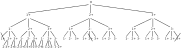
\includegraphics[scale=0.9]{fig_tree_bus_route}
    \end{center}
    \label{fig:tree_bus_route}
\end{figure}

Determining how the tree structure at each level is and how many leafs altogether there are depends on what the load of the bus in a given vertex is, it means, it depends on how many requests are being carried on and how many there are to pick up. The figure \ref{fig:load_bus_scheme} helps to explain the structure of the tree. In the illustration each knot represents the load of the bus in a depth of the tree, how further down it is greater is its respective depth. The edges under a knot tells, how many children with the following load are generated by each vertex with a given load.

\begin{figure}[H]
    \caption{Graph describing the structure of the routes tree}
    \begin{center}
        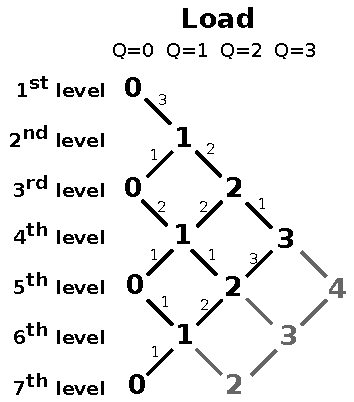
\includegraphics{fig_load_bus_scheme}
    \end{center}
    \label{fig:load_bus_scheme}
\end{figure}

Nevertheless, in order to build a function that allows us to have a mapping from each walk to a natural number, thus enumerating all the possible routes of a bus, is necessary to know, given a depth in the tree how many leafs are under each vertex of this depth. Once this information is available, the transformation function can be computed in a very efficient way.

From the graph illustrated in the figure \ref{fig:load_bus_scheme} it is possible to extract two matrices to represent the structure by denoting the numbers on the edges that leave a knot on the right and on the left in the matrix $Q_{in}$ and $Q_{out}$ respectively. Each column of the matrix $Q_{in}$ has the quantity of children with a larger load to be created by each vertex with a given load, the matrix $Q_{out}$ is analogously constructed, with the difference that it carries the quantity of children with a lower load in the next stage. In addition, each row corresponds then to a load of the bus, beginning from $0$ in the first row to $n$ in the last row, be $n$ the number of requests. Note that, for the generalization it is assumed that a bus can at a moment be carrying all the requests to him assigned. Further constraints should be checked in a future procedure, in order to decide whether a route is feasible according to the input. Knowing that there are $n$ requests implies that there are $2n$ columns, since every request must be picked up and delivered. The mentioned matrices for the figure \ref{fig:load_bus_scheme} are as follows represented.

$$
Q_{in} = 
\begin{bmatrix}
3 & 0 & 2 & 0 & 1 & 0\\
0 & 2 & 0 & 1 & 0 & 0\\
0 & 0 & 1 & 0 & 0 & 0\\
0 & 0 & 0 & 0 & 0 & 0
\end{bmatrix}
,
Q_{out} = 
\begin{bmatrix}
0 & 0 & 0 & 0 & 0 & 0\\
0 & 1 & 0 & 1 & 0 & 1\\
0 & 0 & 2 & 0 & 2 & 0\\
0 & 0 & 0 & 3 & 0 & 0
\end{bmatrix}
$$

An iterative algorithm with these two matrices as input yields a new matrix, which shows, for each depth of the above shown routes tree, the number of vertices for each bus load.

\begin{algorithmic}
\Function{Generate Matrix of Knots Per Load and Depth}{$Q^{in}, Q^{out}$}
\State Let $n$ be the the number of requests and $\odot$ the element-wise multiplication
\State $\displaystyle Q_{2n+1} \gets \begin{bmatrix}1\\ 0 \\ \vdots \\0 \end{bmatrix}$
\For{$i = 2n : 1$}
	\State $\displaystyle Q_{i} \gets Q^{in}_{i} \odot \begin{bmatrix}Q_{i+1,1..n-1} \\ 0\end{bmatrix}
	+ Q^{out}_{i} \odot \begin{bmatrix}0\\ Q_{i+1,2..n}\end{bmatrix}$
\EndFor
\State \Return $Q$
\EndFunction
\end{algorithmic}

The result of applying the function for the shown matrices $Q_{in}$ and $Q_{out}$ is shown below. This provide additionally a new information about the size of the domain which the component of the vector find feasible values, namely in $Q_{1,1}$, since it tells the total number of leafs in the tree. It is useful for constraints check and for a fast creation of the initial generation of fireflies.

$$
Q = 
\begin{bmatrix}
90 & 0 & 6 & 0 & 1 & 0 & 1\\
0 & 30 & 0 & 3 & 0 & 1 & 0\\
0 & 0 & 12 & 0 & 2 & 0 & 0\\
0 & 0 & 0 & 6 & 0 & 0 & 0
\end{bmatrix}
$$

With help of these three matrices and given a correspondent vector component value, the path of a bus can be computed by a transformation function. Below is shown a function that takes these arguments and delivers a path performed by a bus, where its elements do not represent the requests themselves, but the knots of the walk in the tree, which is relative to each bus. A mapping to the absolute requests can be trivially done, once the requests assigned to each bus are known.

\begin{algorithmic}
\Function{Transform component to a cycle in the graph}{$Q^{in}, Q^{out}, Q, x$}
\State Let $n$ be the the number of requests of the bus
\State $Path \gets [ ]$
\State $row \gets 0$
\State $pointer \gets 0$
\For{$col = 1 : 2n$}
	\State $\displaystyle ChildrenSizes = \begin{bmatrix}\underbrace{Q_{row-1,col+1}}_{Q^{out}_{row,col} times}
			\\ \underbrace{Q_{row+1,col+1}}_{Q^{in}_{row,col} times}\end{bmatrix}$
	\For{$child = 1 : Q^{in}_{row,col} + Q^{out}_{row,col}$}
		\If{$x - pointer < ChildrenSizes_{child}$}
			\If{$child < Q^{out}_{row,col}$}
				\State $row \gets row - 1$
			\Else
				\State $row \gets row + 1$
			\EndIf
		\Else
			\State $pointer \gets pointer + ChildrenSizes_{child}$
		\EndIf
	\EndFor
	\State $Path_{col} \gets child$
\EndFor
\State \Return $Path$
\EndFunction
\end{algorithmic}

\subsection{Distance}
For reasons of efficiency of the implementation and numerical error the Manhattan distance can be used to approximate the distance between two vectors in the search space. The Manhattan distance can be described as follows:

$$d(\mathbf{p},\mathbf{q}) = \parallel \mathbf{p} - \mathbf{q} \parallel = \sum_{i=1}^{n} \mid \mathbf{p}_{i}-\mathbf{q}_{i} \mid$$

\subsection{Attractiveness}
As proposed by \textcite[p. 173]{yang_firefly_2009} the attractiveness is calculated with the following quotient, which varies with the squared distance between two vectors.
$$\beta(r) = \frac{\beta_{0}}{1 + \gamma r^2}$$
However, without loss of quality in the method, the attractiveness can be set to vary directly with the distance as the search space is too large and concerns with numerical errors play a important role. So the function is rewritten as follows.
$$\beta(r) = \frac{\beta_{0}}{1 + \gamma r}$$

\subsection{Randomization Term}
The random term of the metaheuristic movement equation is by default $\alpha \cdot \epsilon$, where $\epsilon \sim N(0,1)$. Though, as stated by \textcite[p. 80]{yang_firefly_2010}, \emph{”it is a good idea to replace $\alpha$ by $\alpha S_k$ where the scaling parameters $S_k (k=1,...,d)$ in the $d$ dimensions should be determined by the actual scales of the problem of interest”}. As the size of each dimension are easily obtainable, they are used in this model. Moreover, \textcite[p. 37-38]{yang_firefly_2013} presents an iterative change of the alpha parameter, by turning it variable to the optimization evolution $t$. Thus, he introduces a new variable delta and that parameter is updated by the equation
$$ \alpha_t = \alpha_{t-1} \cdot \delta, (0 < \delta < 1),$$ where $\alpha_0$ is the initial scaling factor. The author gives also an advice about setting delta: \emph{”$\delta$ is essentially a cooling factor. For most applications, we can use $\delta = 0.95$ to $0.97$”}.

At last, it is wanted a integer number for the stochastic term, as the search space is discrete. In order to achieve that, rounding is performed, proper concerns about numerical errors should be taken in the implementation, so that they are reduced at most.

\subsection{Movement in the Discrete Space}
The movement of a firefly $i$ towards $j$ is determined by $$\mathbf{x^{t+1}_i} = \mathbf{x^{t}_i} + \beta(d(\mathbf{x^{t}_i}, \mathbf{x^{t}_j})) \cdot (\mathbf{x^{t}_j} - \mathbf{x^{t}_i}) + RandomTerm(t)$$
As the fireflies move in a discrete vector space, the terms of the sum should be also integer number. Since $\beta$ is less or equal than one and its image is the set of the real numbers, the equation can be modified, by turning the multiplication into a division by the inverse function and by rounding the result of the function $\beta$, or rather, implementing it, so that its image is the set of the natural numbers.
$$\mathbf{x^{t+1}_i} = \mathbf{x^{t}_i} +  \lfloor \frac{(\mathbf{x^{t}_j} - \mathbf{x^{t}_i})}{\beta^{-1}(d(\mathbf{x^{t}_i}, \mathbf{x^{t}_j}))} \rfloor + RandomTerm(t)$$

AND WHEN IT IS OUT OF DOMAIN? WHAT TO MAKE?

\subsection{Intensity Function}
The intensity function models the brightness of a firefly and should be directly proportional to the utility function of the problem to be maximized. However, the problem's goal is to minimize the operation costs, and in the Firefly Algorithm it is not enough utilizing the negative costs function instead, since the intensity function is by definition non-negative.

Nevertheless, the costs function has an lowest possible value, that can be estimated. Here it is proposed to sum the $v$ most distance vertices in the requests graph, so that $v$ is twice the number of requests, since every request has two correspondent vertices, one for getting in and one for getting out. Once this value is calculated, the costs of a given solution can be subtracted from it, in order to obtain an utility function. The process is equivalent to translating the function.

Let $m$ be the mentioned superior limit for the costs, $f$ a function that tells in a binary matrix which edges are visited by a solution vector and $C$ the adjacency matrix of the requests graph with the costs between any one of them, then the intensity can be defined like in the following formula.

$$I(\mathbf{x}) = \begin{cases} 0 & \text{if }\mathbf{x}\text{ does not meet the constraints}\\
								m - \displaystyle\sum_{i=1}^{2n+1}\sum_{j=1}^{2n+1} f(\mathbf{x})_{i,j} \cdot C_{i,j} & \text{else}
					\end{cases}$$

\subsection{Initial Solution}
A initial set of feasible solutions is calculated by simply generating random natural numbers in an interval to each component of the vector. Firstly, the first component is randomized, its range is $[0, k^n)$, where there are $n$ requests and $k$ buses. Secondly, the other components are randomized, their domain intervals are determined based on the distribution of requests to buses resulted from the first component randomization. So the first generation of fireflies can be efficiently created. [ARE THEY FEASIBLE WHEN THE BUSES HAVE LIMIT OF PASSENGERS? OR TIME CONSTRAINTS? NO!]

\subsection{Parameters}
The choice of the parameters is basically based on the work of \textcite[p. 37-38]{yang_firefly_2013}. For that the scale $L$ of the problem is taken into consideration, it represents the size of the search space and is calculated by multiplying the sizes of the intervals, in which the intensity function is defined, of each dimension. The parameter gamma is then set $\gamma = 1/\sqrt{L}$. In order to have an broad exploration of the space it is set $\alpha_0 = 0.1$, the parameter is reduced along the optimization process. Lastly, it is set $\beta_0 = 1$, $\delta = 0.95$ and the number of fireflies to 40.

\subsection{Two-Phase Optimization}
It is to note in a regular problem instance that the distribution of requests to bus has a greater weight it the cost function. Empirical observations suggest that this distribution is roughly the most determinant factor in the calculation of the costs. For instance, the grouping requests that are geographically near tends to show better results regardless of the route. Yet, the route of each bus plays an important role in finding an optimal result.

Moreover, as the contribution to the cost function by the vector components that describe the routes is strongly dependent on the distribution of requests to each bus, it makes no sense trying to optimize these components if this assignment varies strongly in the cost minimization procedure.

On the basis of these observations, an optimization process with two phases is advised. In this schema, there is a first stage, where only the first vector component is optimized by moving the fireflies only in this dimension of the search space. In a second stage, the other components are optimized by anchoring the first component and allowing the movement of the fireflies in these other dimension.

[PICTURE SHOWING PROGRESS OF THE ITERATIONS]

\subsection{Implementation}
One of the main difficulties in implementing the algorithm is with the large that the numbers may have. To workaround the problem the programming language Python\footnote{\url{https://www.python.org/}} was chosen, since it has a native implementation of unlimited integers. Besides, the proposed model has a considerable quantity of matrix operations, therefore, the libraries NumPy\footnote{\url{http://www.numpy.org/}} and Scipy\footnote{\url{http://www.scipy.org/}} were used for that purpose. For drawing the graphs the was adopted library Matplotlib\footnote{\url{http://matplotlib.org/}}, which has an easy-to-use interface for the programmer.

Care by the numerical operations and data type had to be specially taken to ensure no capacity overflows and a controlled numerical error at a lowest level.

To obtain a better performance and the most recent implemented features it is required that the implementation program runs on the newest possible tool versions. Namely, it was developed on the versions 3.3 of Python, 1.10 of the NumPy, 0.16 of the SciPy and 1.3 of the Matplotlib.

- Input (Manual,help)

\chapter{Evaluation}
- Method for evaluation

- Experiments Setup

- Dataset

- Results

- Comparison

\chapter{Conclusion}
- Further Research

% e aqui vai a parte principal
% 
% \chapter{Estado da arte}
% \chapter{Mais estado da arte}
% \chapter{A minha contribuição}
% \chapter{Prova de que a minha contribuição é válida}
% \chapter{Conclusão}

% referências
% aqui será usado o environment padrao `thebibliography'; porém, sugere-se
% seriamente o uso de BibTeX e do estilo abnt.bst (veja na página do
% UTUG)
% 
% observe também o estilo meio estranho de alguns labels; isso é
% devido ao uso do pacote `natbib', que permite fazer citações de
% autores, ano, e diversas combinações desses

\nocite{*}
%\bibliographystyle{abntex2-alf}
\printbibliography

\end{document}
